%!TEX root = ../main.tex %%%%%%%%%%%%%%%%%%%%%%%%%%%%%%%%%% Links:
%https://www.yumpu.com/en/document/read/7789379/lowest-common-ancestorlca-chair-for-efficient-algorithms
%
% Difficulty: Companies: 
%%%%%%%%%%%%%%%%%%%%%%%%%%%%%%%%%%

\chapter{Distance between nodes in BST}
\label{ch:distance_between_nodes_in_tree}
\section*{Introduction}

In the problem described in this chapter  we are going to investigate how we can find the the
distance between two nodes in a binary search tree. As we will see this problem can be approached
and solved very straightforwardly if we are able identify the key idea behind it. This insight can
become apparent after we look at a few examples and our advice for approaching this problem (and to
be honest all problems on graphs and trees) is to draw and discuss quite a few examples with your
interviewer. This help you get a much better intuitive understanding of what the problem is really
about, which will eventually lead to the eureka moment.

This is going to be a relatively short chapter because the solution is built on top of the solution
of a problem discussed in another chapter. In Section
\ref{sec:distance_between_nodes_in_tree:problem} we will have a look at the formal problem statement
and in Section \ref{distance_between_nodes_in_tree:sec:discussion} we discuss the solution approach
and we will look into two possible different implementations: recursive and iterative. 

\section{Problem statement}
\label{sec:distance_between_nodes_in_tree:problem}
\begin{exercise}
	Write a function that takes as input a binary search tree $T$ and two nodes $p$ and $q$ and
	returns the distance between $p$ and $q$. The distance between two nodes $D(p,q)$ is defined as
	the number of edges you need to traverse to get from $p$ to $q$.
	
	\begin{example}
		\hfill \\
		Given the tree shown in Figure \ref{fig:distance_between_nodes_in_tree:example1}, $p = 1$
		and $q=3$, the function returns $D(1,3)=2$ 
		
		If $p=3$ and $q=2$ the function returna $1$.
	\label{ex:distance_between_nodes_in_tree:example1}
	\end{example}

	\begin{example}
		\hfill \\
		Given the tree shown in Figure \ref{fig:distance_between_nodes_in_tree:example2}, $p = 5$
		and $q=2$, the function returns $D(5,2)=6$ 
		\label{ex:distance_between_nodes_in_tree:example2}
	\end{example}
\end{exercise}

\section{Clarification Questions}

\begin{QandA}
	\item \begin{questionitem} \begin{question} Can $p$ be equal to $q$?  \end{question} 	 
    \begin{answered}
		\textit{Yes, this is a valid case.}
	\end{answered} \end{questionitem}
	
	\item \begin{questionitem} \begin{question} Is it guaranteed for  $p$ and  $q$ to be present in $T$?  \end{question} 	 
    \begin{answered}
		\textit{Yes, you can assume $T$ always contains both $p$ and $q$.}
	\end{answered} \end{questionitem}

\end{QandA}

\section{Discussion}
\label{distance_between_nodes_in_tree:sec:discussion}
As already mentioned in the introduction this problem can become quite challenging if we are not
able to steer our approach in the right direction. The intuitive idea on how this problem should be
approached is going to be almost self-evident if we look at a couple of examples, solve them by hand
and then try to look for similarities in their solution.

Let's have a look at some instances of this problem and their solution. If we consider $T$ to the
tree depicted in Figure \ref{fig:distance_between_nodes_in_tree:example3} then the distance between
nodes $p=3$ and $q=9$ is $4$ and  
can be found by walking up the tree from node $3$ up to a node $5$ (follow the red arcs) from which
we can descend and reach  node $9$ (green arcs). Notice that node $5$ is the first node from which
we can visit the tree down and reach both nodes $3$ and $9$. You can also see that the same
reasoning applies also to the trees shown in Figures
\ref{fig:distance_between_nodes_in_tree:example4} and
\ref{fig:distance_between_nodes_in_tree:example5} where you get the minimum distance by traveling up
to the first node that allows you to reach the destination node. Notice that in Figure
\ref{fig:distance_between_nodes_in_tree:example5} the path upwards has length zero as from $p$ you
can already reach $q$ by visiting down the tree.

At this point should be clear that the minimum distance between two nodes can be calculated as the
sum of distances from $p$ and $q$ their lowest common ancestor (LCA). The LCA is the lowest node
from which it is possible to walk in a downward direction and reach both $p$ and $q$. In order to go
from $p$ to $q$ one must pass through their LCA. If you need to refresh your memory on the topic of
finding the LCA on binary search trees you can read Chapter \ref{ch:lowest_common_ancestor}. Listing
\ref{list:distance_between_nodes_in_tree} shows a possible implementation of the idea described
above. 

\begin{figure}
	\centering
	\begin{subfigure}[b]{0.5\textwidth}
		\centering
		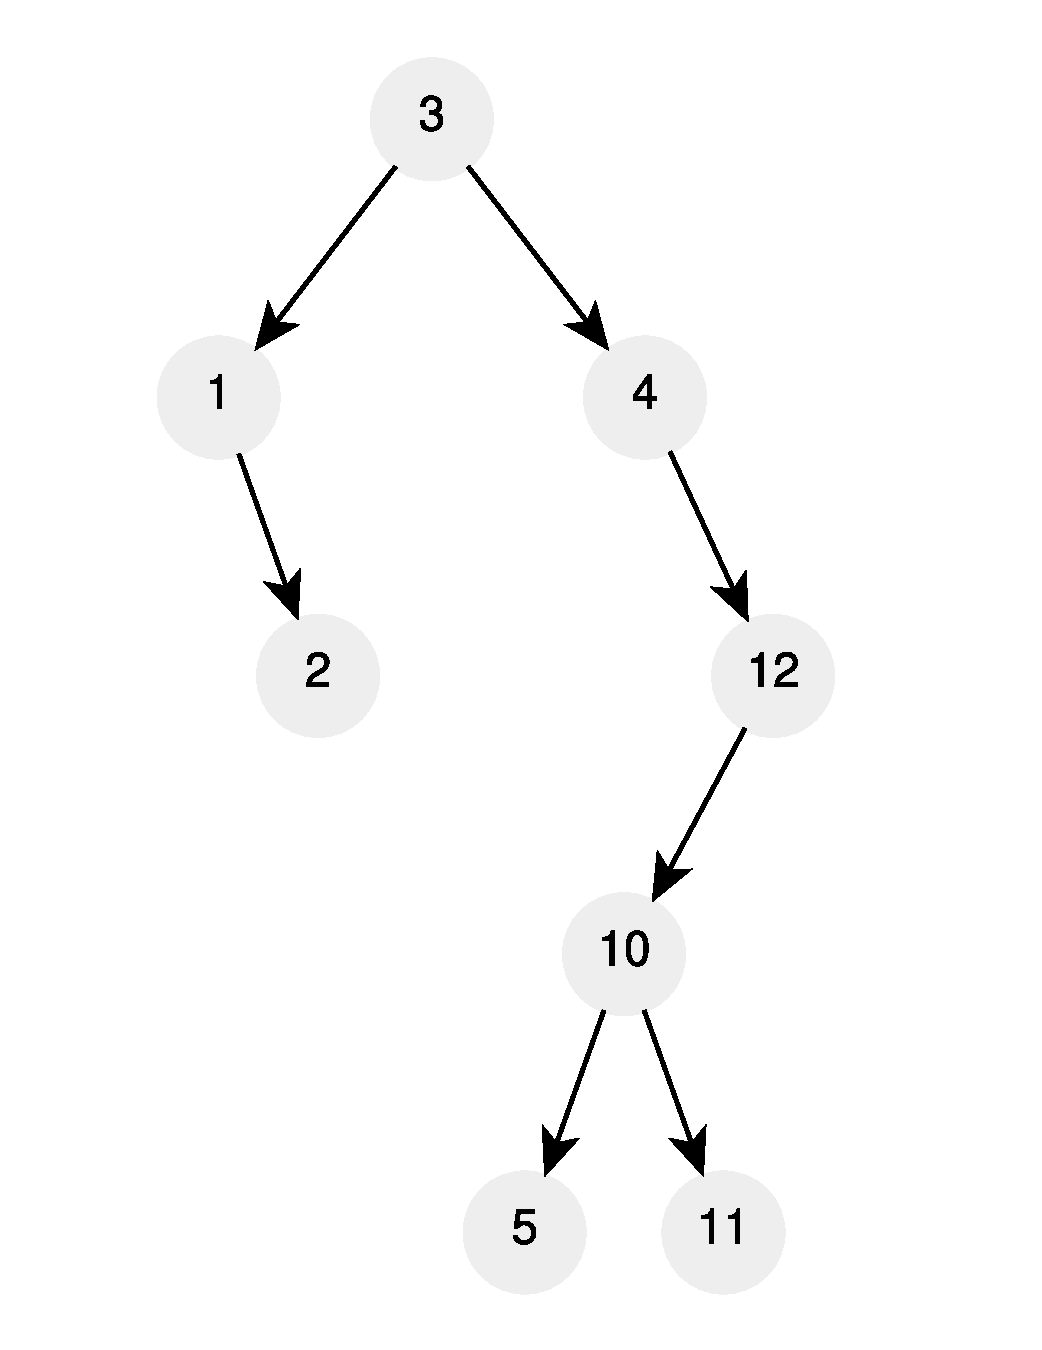
\includegraphics[width=0.8\textwidth]{sources/distance_between_nodes_in_tree/images/example2}
		\caption{Binary Search tree of the Example
		\ref{ex:distance_between_nodes_in_tree:example2}}.
		\label{fig:distance_between_nodes_in_tree:example2}
	\end{subfigure}
	\hfill
	\begin{subfigure}[b]{0.3\textwidth}
		\centering
		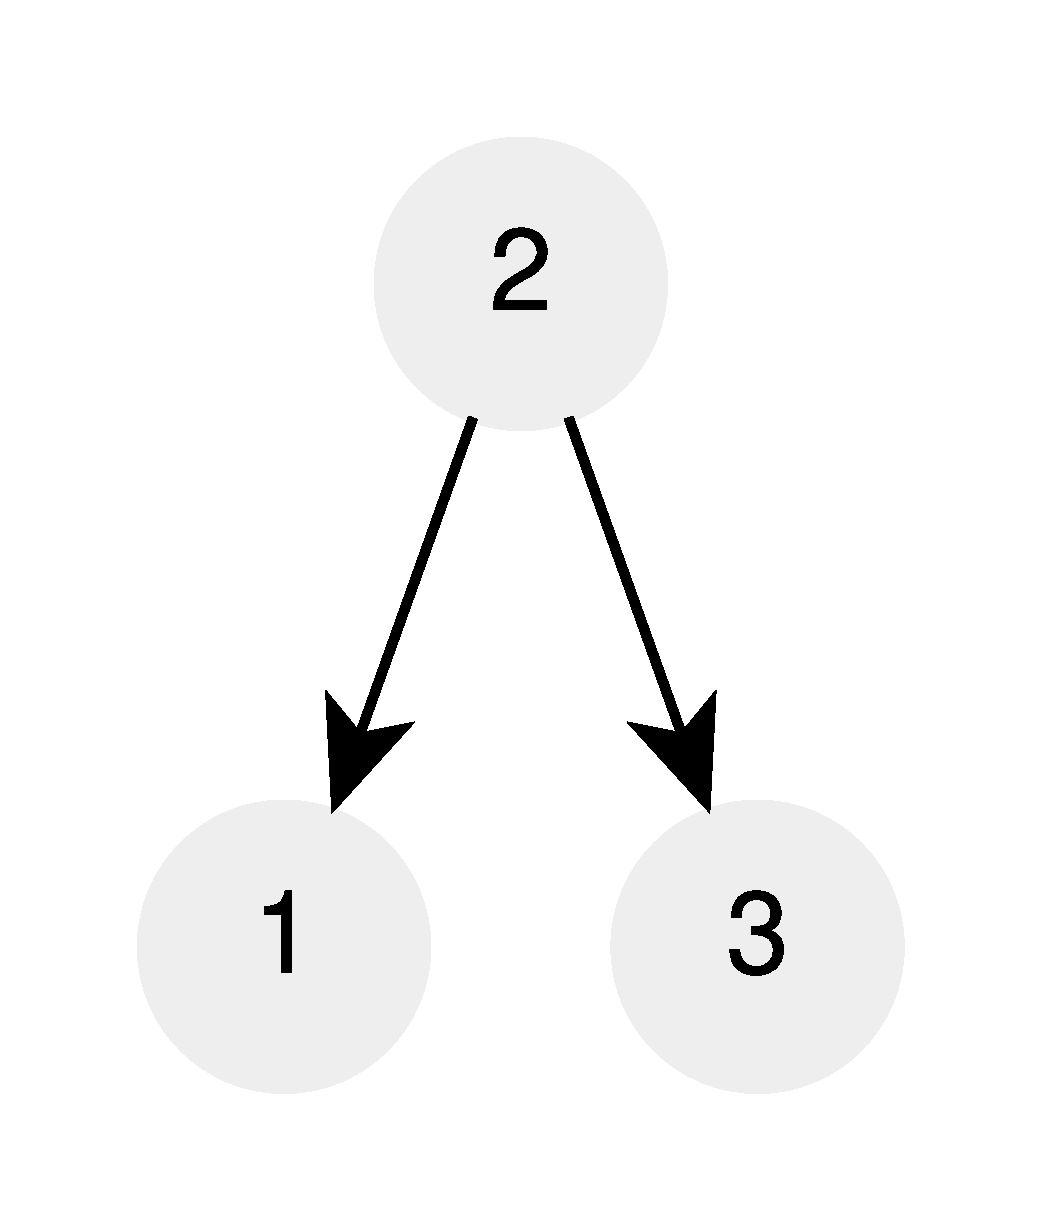
\includegraphics[width=\textwidth]{sources/distance_between_nodes_in_tree/images/example1}
		\caption{Binary Search tree of the Example
		\ref{ex:distance_between_nodes_in_tree:example1}}.
		\label{fig:distance_between_nodes_in_tree:example1}
	\end{subfigure}
	\centering
	\begin{subfigure}[b]{0.3\textwidth}
		\centering
		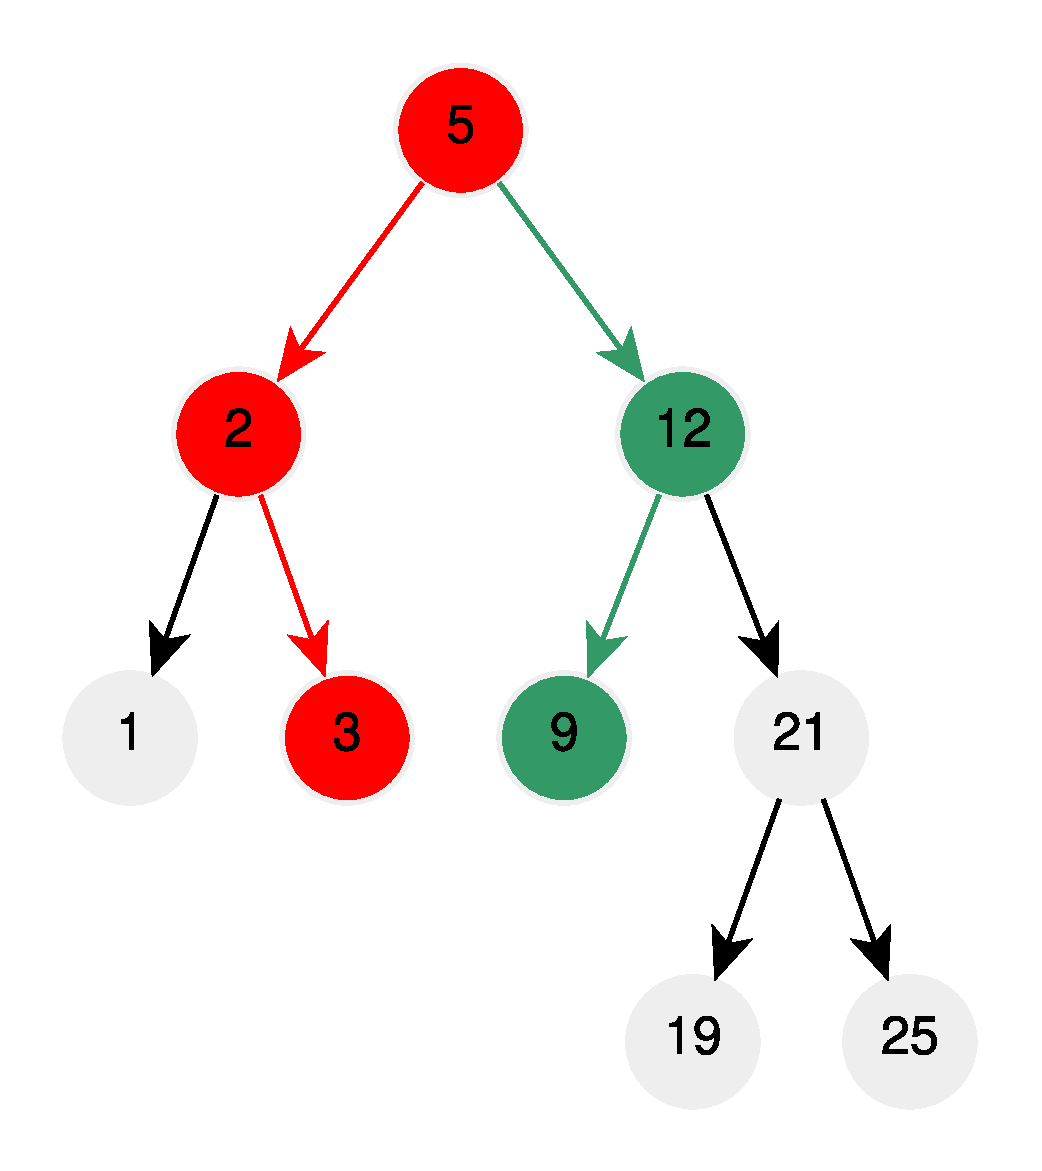
\includegraphics[width=\textwidth]{sources/distance_between_nodes_in_tree/images/example3}
		\caption{}
		\label{fig:distance_between_nodes_in_tree:example3}
	\end{subfigure}
	\hfill
	\begin{subfigure}[b]{0.3\textwidth}
		\centering
		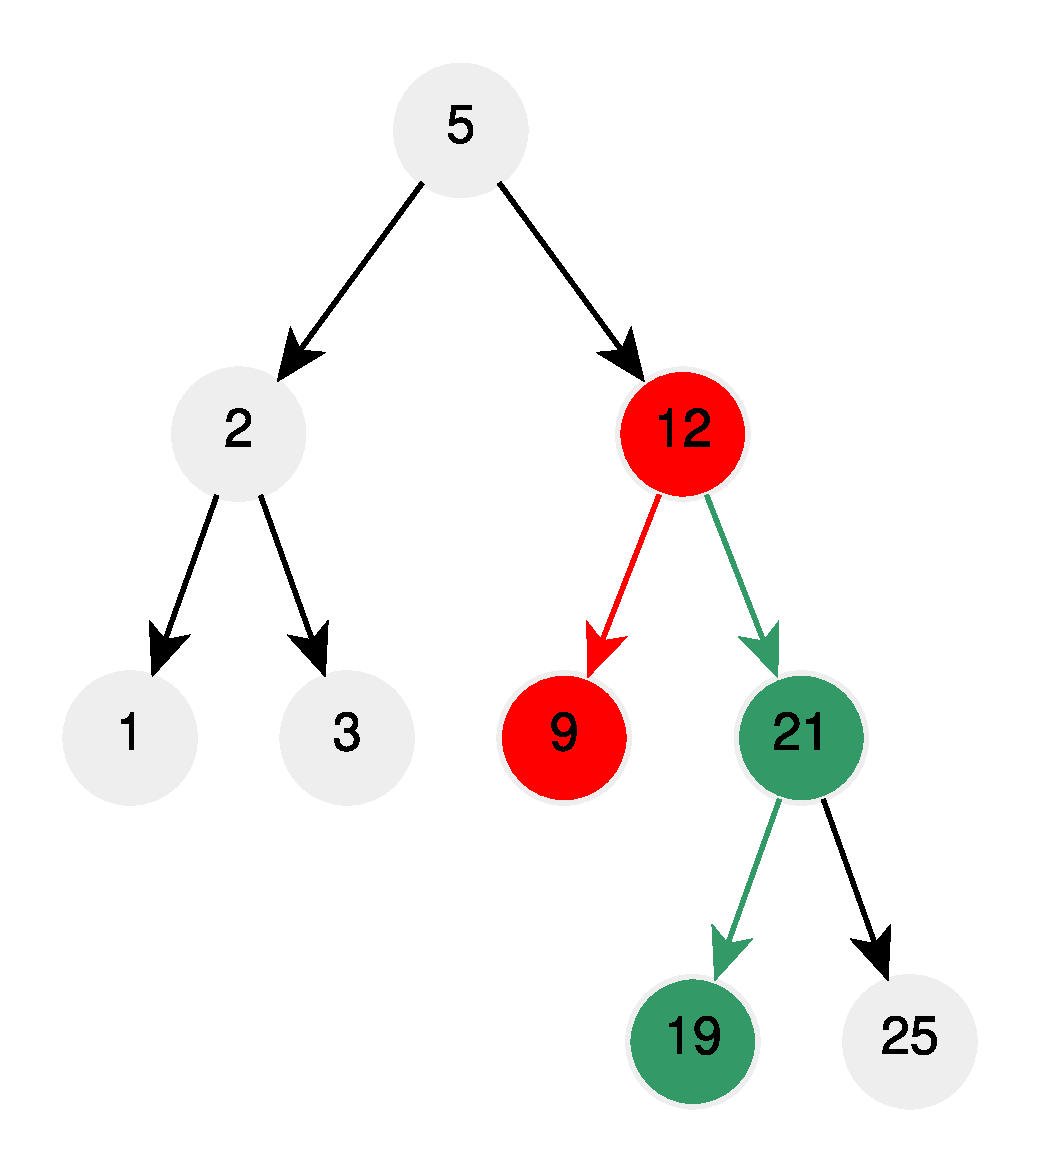
\includegraphics[width=\textwidth]{sources/distance_between_nodes_in_tree/images/example4}
		\caption{}
		\label{fig:distance_between_nodes_in_tree:example4}
	\end{subfigure}
	\hfill
	\begin{subfigure}[b]{0.3\textwidth}
		\centering
		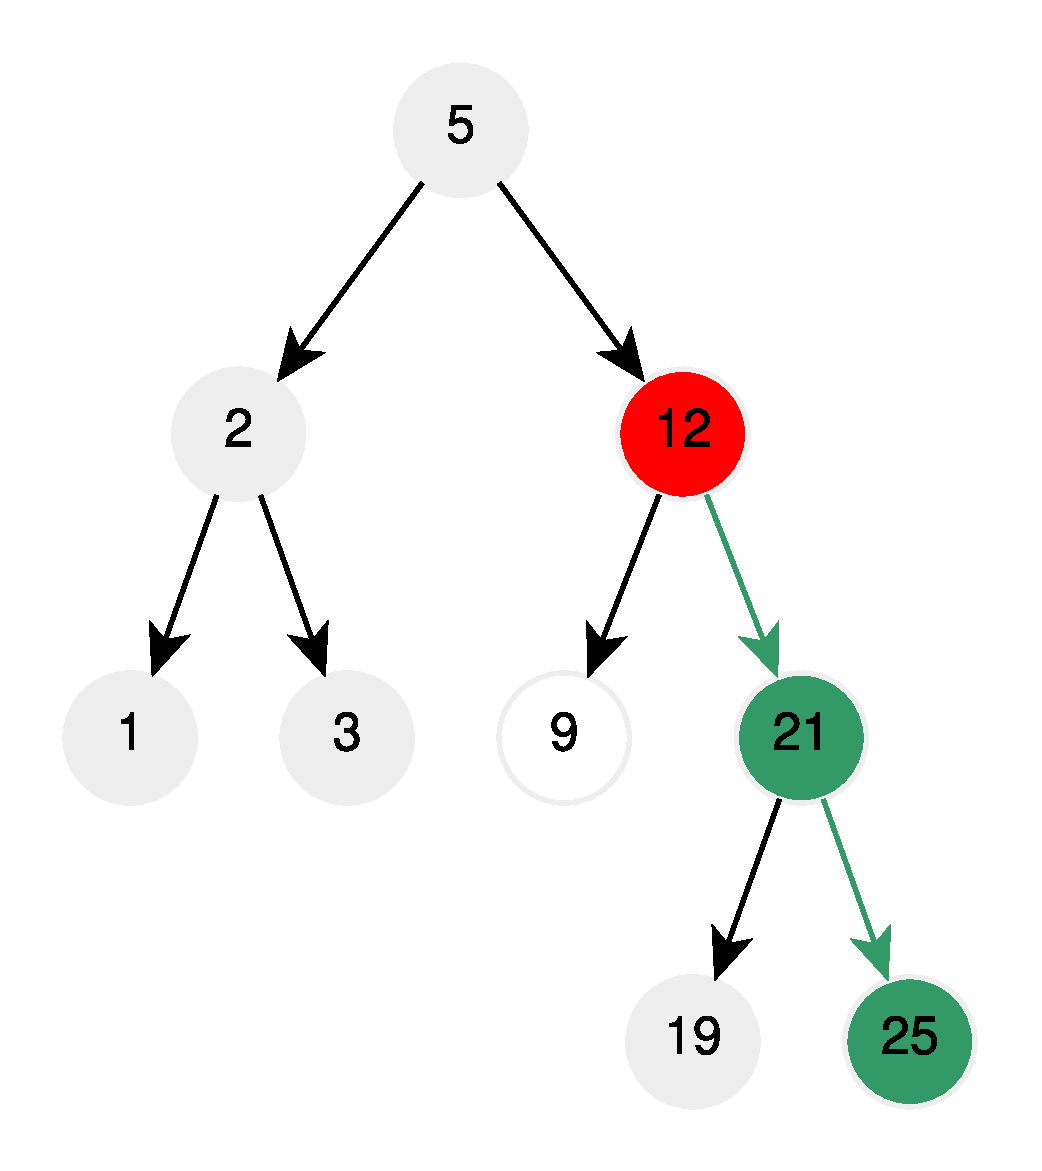
\includegraphics[width=\textwidth]{sources/distance_between_nodes_in_tree/images/example5}
		\caption{}
		\label{fig:distance_between_nodes_in_tree:example5}
	\end{subfigure}
	\caption{Various istances of the problem of finding the distance between two nodes in a BST and
	their solutions. Figures \ref{fig:distance_between_nodes_in_tree:example3},
	\ref{fig:distance_between_nodes_in_tree:example4}, and
	\ref{fig:distance_between_nodes_in_tree:example5} have nodes and arcs in red and green to
	highlight the paths between the $p$ and $q$ and their LCA, respectively.}
\end{figure}



	\lstinputlisting[language=c++, caption={Solution to the problem of finding the distance between two nodes in a binary search tree.},label=list:distance_between_nodes_in_tree]{sources/distance_between_nodes_in_tree/distance_between_nodes_in_tree_solution1.cpp}



\section{Conclusion}
In this chapter we have seen how we can efficiently solve the problem of finding the distance between two nodes in a binary search tree
by using the concept of LCA (discussed more in details in Chapter \ref{ch:lowest_common_ancestor}). The general strategy is that,
we can calculate the distance between the LCA and both $p$ and $q$. The sum of these two distances is the final answer.
The distance between two nodes in a binary search tree can be found by slightly modifying the standard search algorithm for BSTs so that we return
the number of recursive calls made instead of a boolean value signaling whether the element to be searched was found or not.